% schwartz-christoffel stuff
\label{chap-sc}
\section{Introduction}

The example of the Ramsay horseshoe in \secref{intro-FAS} shows that leakage can be problematic for spatial smoothing. \label{cor-3s3}The horseshoe is a rather simple example for leakage, however it does encapsulate the most important feature of leakage: a gap with differing response on each side. It is not so simple to be unrealistic however: comparing the horseshoe to the Aral sea example seen in \secref{intro-GAM}, there are many similarities. Starting with a simple example such as the horseshoe should reveal more fundamental problems without getting bogged-down in issues relating the the overall complexity of the domain. 

Leakage is caused by the smooth not respecting the boundary of the domain of interest, so transforming the domain in such a way that the smoother does not need to respect the boundary should reduce leakage. In the case of the Ramsay horseshoe it seems rather obvious what we would like to do: straightening the domain out to be a rectangle seems like the most logical course of action. Objects within the horseshoe surely experience the domain in this way (i.e. their coordinate system is based on the major and minor axes of the shape, rather than Cartesian coordinates) and within-domain distances are well approximated by a rectangle with length equal to the major axis length of the horseshoe and width the same as the horseshoe. As we shall see through the rest of the chapter, the \sch\ transform allows for exactly such a morphing of the domain.

This chapter investigates the efficacy of using a conformal mapping to transform the domain in which we wish to perform smoothing. The mapping takes points in the domain of the data ($W$, which is the interior of $\Gamma$\label{cor-3s1-3}) to a domain on which it is easier to smooth ($W^*$). In particular the utility of the \sch\ transform is examined (elaborating on \cite{eilerstalk}).

Given some region that it is difficult to smooth over, one approach is to transform the domain in which the problem resides to some known shape. So, for example, one could transform a region into a rectangle, circle or other familiar shape to avoid leakage via a mapping. Figure \ref{mappingdia} shows $\varphi$ mapping from the rectangle to an arbitrary shape and $\varphi^{-1}$ mapping in the other direction\label{cor-3s4-2}. It seems natural to treat the domain as if it were made of silly putty and simply squash the region into the shape required to perform analysis, especially in the case of the Ramsay horseshoe. A transformation-based approach is appealing since it allows the use of existing techniques in the transformed domain; once it's a familiar shape, the domain can be smoothed using a splines just as one would when the domain does not have a complicated boundary.

%% Simple diagram showing the mapping
%\begin{figure} [t]
%\centering
%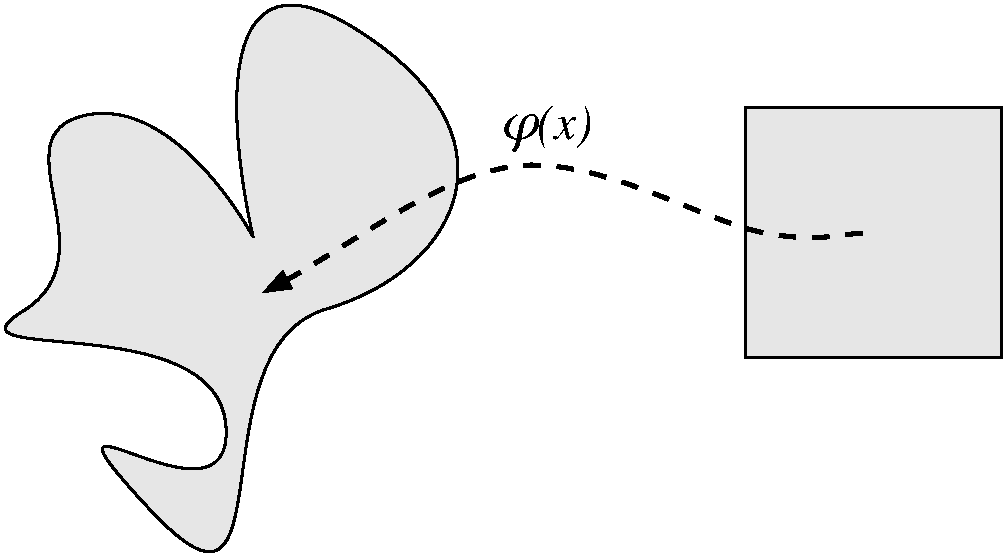
\includegraphics[scale=0.3]{sc/figs/simpledia.pdf}
%\caption{An example of a transformation; the function $\varphi$ takes the points in the rectangle and maps them to the region on the left.}
%\label{simpledia}
%\end{figure}

% Mapping diagram from my whiteboard
\begin{figure} [t]
\centering
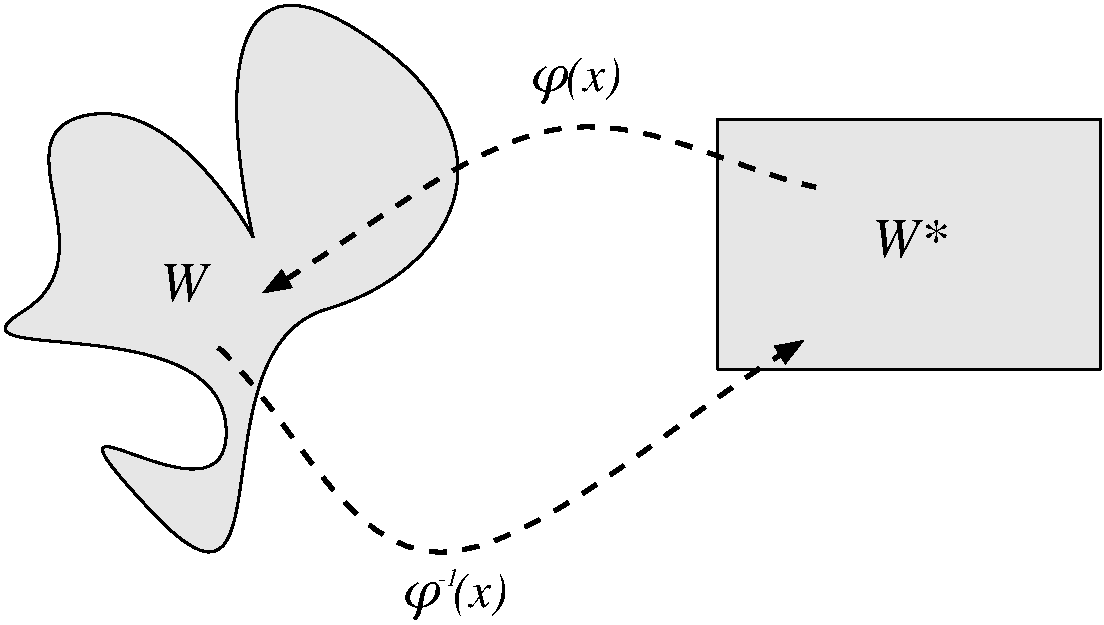
\includegraphics[scale=0.5]{sc/figs/mappingdia.pdf}
\caption{Diagram showing the $\varphi^{-1}$ mapping from an arbitrary shape ($W$; where the data were collected) to the rectangle ($W^*$; where smoothing can be performed reliably). $\varphi$ maps from the rectangle to the arbitrary shape. $\varphi$ and $\varphi^{-1}$  will be referred to as the forwards and backwards mappings respectively (c.f. \secref{schparprob}).\label{cor-3s4}}
\label{mappingdia}
\end{figure}

The \sch\ mapping takes a specified shape and maps it to an arbitrary polygon\label{cor-3s6}. The most common domains to transform from are: (i) the upper half-plane, (ii) a rectangle and (iii) the unit disc. This is achieved in the upper half-plane case by taking points on the real line and mapping them to the vertices of the polygon (see \fig{reallinedia}). This can be thought of as ``unwrapping'' the polygon onto the real line. For the unit disc case, points on the circle bounding the unit disc map to vertices on the polygon (see \fig{unitdiskdia}). The rectangular case is somewhat similar to the unit disc in that extra points are added to the boundary. Once the mapping has been performed, those points lying inside the polygon are also moved around, creating a new (non-uniform) distribution of space. These three domains are discussed in more detail in \secref{schparprob}.

% Diagram showing upper half plane to polygon
\begin{figure} [t]
\centering
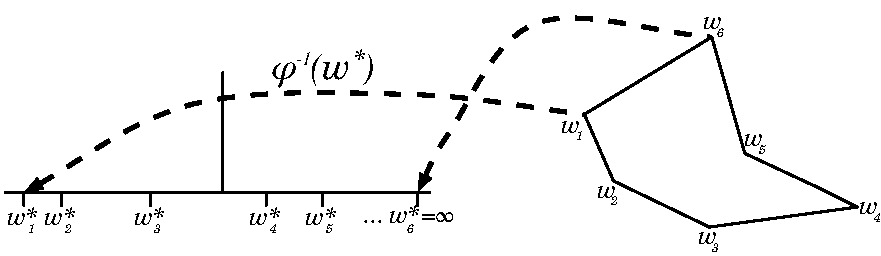
\includegraphics[scale=0.6]{sc/figs/reallinedia.pdf}
\caption{\label{cor-3s5}An example of mapping and arbitrary point from the upper half-plane to a point on a polygon (solid line). Dashed lines show the inverse map of the vertices of the polygon ($w_k$) to the prevertices ($w^*_k$) via $\varphi^{-1}$ for $k=1$ and $k=6$. Note that $w_6$ is mapped to $\infty$ on the real line.}
\label{reallinedia}
\end{figure}

% Diagram showing unit disc to polygon
\begin{figure} [t]
\centering
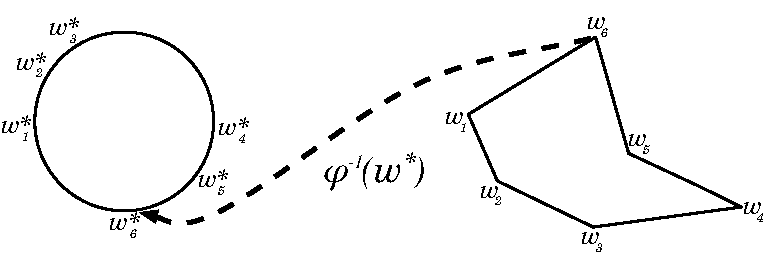
\includegraphics[scale=0.6]{sc/figs/unitdiskdia.pdf}
\caption{\label{cor-3s7}An example of mapping an arbitrary point on the unit disc to a point on a polygon (solid line). The dashed line shows the inverse map of one of the vertices of the polygon ($w_6$) to its corresponding prevertex ($w^*_6$) via $\varphi^{-1}$.}
\label{unitdiskdia}
\end{figure}

\subsubsection{Proposed procedure}

The central idea here is to transform the domain with the complicated boundary to one that is less complicated, then smooth in this transformed domain. The procedure is as follows:

\begin{enumerate}
\item Determine the domain over which we would like to smooth, $W$. This could be the polygon which bounds the region or a simplified version of it\label{cor-3s8-1}.
\item Compute the \sch\ transform of $W$ (the domain with the complicated boundary) to get $W^*$ (the nicely shaped domain, in which we want to smooth). We then obtain the functions $\varphi$ and $\varphi^{-1}$, which map between the two domains\label{cor-3s8-2}.
\item Map the co-ordinates of the data in $W$ to $W^*$, via $\varphi^{-1}$\label{cor-3s8-3}.
\item Smooth the data in $W^*$ using the methods in chapter \ref{chap-intro}.
\item Transform back to $W$; perform any further inference, create heatmaps, etc\label{cor-3s8-4}.
\end{enumerate}

The second section of this chapter explains the technical details of the mapping. The third section gives results of some simulations and the final section summarizes the results of these simulations and draws conclusions about the utility of the method.

\section{Technical details}

This section gives some of the mathematical and computational details required to calculate the \sch\ mapping. The primary reference is \citeb{driscoll}, which covers almost all aspects of the \sch\ transform.

\subsection{Nomenclature}
\label{sc-nomen}

The polygon is first defined formally along with its associated quantities, as they will be referred to throughout the rest of the chapter.

A polygon, $\Gamma$, is a collection of vertices $w_1, w_2,\ldots,w_K$ and interior angles $\alpha_1\pi, \alpha_2\pi, \ldots, \alpha_K\pi$. For convenience define $w_{K+1} = w_1$ and $w_0=w_K$. Numbering of vertices is anti-clockwise. The angles are such that $\alpha_k \in (0,2]$ and we require:
\begin{equation}
\sum_{k=1}^K (1-\alpha_k) = 2.
\end{equation}
The external angle, $\theta_k\pi$, is given by $(1-\alpha_k)\pi$ (see \fig{anglediagram}). 

% Diagram showing the exterior/interior angle relationship.
\begin{figure} [t]
\centering
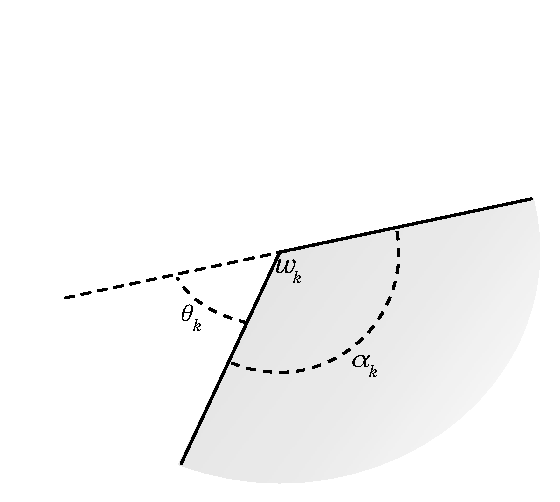
\includegraphics[scale=0.6]{sc/figs/anglediagram.pdf}
\caption{\label{cor-3s9}The internal angle $\pi\alpha_k$ is associated with the vertex $w_k$. The external angle is $\pi\theta_k$. Shading indicates the inside of the polygon.}
\label{anglediagram}
\end{figure}

\label{cor-r29-1}
Both points in the domain and the vertices of the polygon are represented as complex numbers (e.g. for some point $w$,  $w=x_1+ix_2$). The boundary of the polygon is denoted by $\Gamma$. Two domains have already been mentioned: $W$ and $W^*$, denoting the original domain (inside $\Gamma$) and the transformed domain (for example, the plane, unit disc or rectangle\label{cor-3s10}), respectively. The vertices of $\Gamma$ are denoted as $w_k$ and the vertices of the transformed boundary are denoted as $w^*_k$ (the \emph{prevertices}). In general, a point in the polygon's original domain will be denoted as $w$ and in the transformed domain as $w^*$. 

The function $\varphi$ is a mapping from the transformed domain to the polygon (i.e. $\varphi:W^* \mapsto W$). The inverse mapping function, $\varphi^{-1}$, is used to take points from the polygon to one of: the unit disc, rectangle or half-plane (\label{cor-3s11}$\varphi^{-1}:W \mapsto W^*$).  See \fig{mappingdia}.

% mappingdia was here!

\subsection{\sch\ Mapping}
\label{schparprob}
There are many possible domains that can be mapped from (see \cite[section 4]{driscoll} for \label{cor-3s12}many examples). This section looks at the mathematical formulation for the upper half-plane, unit disc and rectangle. The three mappings discussed here are either canonical (in the case of the half-plane) or considered to be useful in a smoothing context (the other two).

For the purposes of smoothing we are interested in the function $\varphi^{-1}$ (i.e. the function that goes from the domain in which the data were collected to the transformed one), $\varphi$ must be found before calculations can be made with its inverse (see \secref{sc-backwardsmap}). In the literature $\varphi$ is referred to as the \emph{forwards map} and $\varphi^{-1}$ as the \emph{backwards map}.

The forwards map, $\varphi$, is determined up to translation, scaling, and rotation by the prevertices (see below). \label{cor-3s13-1}The \emph{\sch\ parameter problem} is the task of efficiently finding the prevertices (hence $\varphi$). This is a complex problem since the prevertices are solutions to non-linear equations. The \sch\ parameter problem is discussed in \secref{sc-mapping-problem}. For the rest of this section the prevertices (the $w^*_k$s) are assumed to be known. 

The rest of the section discusses the mathematical form of the mappings for the upper half-plane, unit disc and rectangle. In each case the mapping takes the form of an integral which must be evaluated numerically (since there are not closed-form solutions). Accurate and fast (since often many evaluations are needed) computation of these integrals is covered in \citeb[pp. 27--29]{driscoll} and \citeb{howell90}. Methods for finding and computing \sch\ transformations are implemented in the \textit{SC Toolbox} package for MATLAB written by Tobin A. Driscoll\label{cor-soft2}.

\subsubsection{The upper half-plane}
\label{sc-parprob}

When mapping from the upper half-plane\label{cor-3s14-1} to $W$\label{cor-3s1-1}, first set $\varphi(\infty) = w_K$ without any loss of generality. \citeb[p. 10]{driscoll} then give the following formula:
\begin{equation}
\varphi(w^*) = A + C \int^{w^*}_{w^*_0} \prod_{k=1}^{K-1} \left (\zeta-w^*_k \right )^{\alpha_k-1} d\zeta.
\end{equation}
Here $A$ and $C$ are complex constants determined once the $w^*_k$ (which all lie on the real line\label{cor-3s13-2}) have been calculated. These control the scaling, translation, and rotation of the transform. 

Mathematically, the base point of the integration does not matter, as it only affects the value of $A$ (\cite[p. 3]{driscoll}).\label{cor-3s14-3} However, when calculating $\varphi(w^*)$ numerically, $w^*_0$\label{cor-3s14-2} is usually chosen to be the prevertex nearest to the point $w^*$. This is primarily to avoid numerical problems (such as avoiding singularities, see \citeb[p. 27-29]{driscoll}) but choosing a $w^*_0$ near to $w^*$ also makes the computation faster.

Although setting $\varphi(\infty) = w_K$ does not make any difference in a mathematical sense, it does mean that the density of the points mapped into the upper half-plane is rather odd from a smoothing perspective. Given two adjacent points near $w_K$, their spacing on the upper half-plane is huge (since $w_K$ is mapped to $\infty$) in comparison to two adjacent points \label{cor-e6}near any other vertex. For this reason mapping from the upper half-plane is not pursued further here.

\subsubsection{Unit disc}

The formula for the unit disc looks very similar to that for the upper half-plane but the product now runs over all $K$ prevertices (which are complex numbers, \citeb{driscoll96})\label{cor-3s13-3}. The integrand is simply a constant multiple of the upper half-plane case (see also \cite[p. 12]{driscoll}):\label{cor-e5}
\begin{equation}
\label{unitscmap}
\varphi(w^*) = A + C \int^{w^*}_{w^*_0} \prod_{k=1}^{K} \left (1 - \frac{\zeta}{w^*_k} \right )^{\alpha_k-1} d\zeta.
\end{equation}
As above, $A$ and $C$ are complex constants responsible for scaling, translation, and rotation, and $w^*_0$ is the base point of the integration.

\subsubsection{Rectangle}
\label{cor-3s13-4}\label{cor-3s15-2}\label{cor-r29}\label{cor-r29-4}\label{cor-r29-5}\label{cor-r29-2}

The rectangle mapping is slightly different in its calculation to the two above mappings. The mapping proceeds in two stages: first mapping from the rectangle to the upper half-plane and then mapping from upper half-plane to $W$ can be calculated (prevertices lie on the real line, as described for the upper half-plane case). 

For the rectangle case, the four vertices of $\Gamma$ which will correspond to the four corners of the rectangle must be specified. The mapping from the rectangle to the upper half-plane is exactly defined by the Jacobi elliptic sine function, $\text{sn}$ (further information may be found in \citeb[p. 701]{handbuch}, \citeb[p. 567--586]{aands} and the appendix of \citeb{howell90}). The Jacobi elliptic sine function maps the corners of the rectangle to the points $-\gamma^{-1/2}$, $-1$, $1$ and $\gamma^{1/2}$ on the real line (these are marked in order as $A$, $B$, $C$ and $D$ in figure \ref{rectangledia}). $\gamma$ is defined by the aspect ratio of the rectangle and hence which corners of the rectangle map to which vertices of $\Gamma$ (the computation is covered in depth in the appendix of \citeb{howell90} and \citeb[p. 50]{driscoll}). We now have $\text{sn}$ which maps from the rectangle to the upper half-plane, so all that is required is to fine the \sch\ mapping from the upper half-plane to the polygon, $W$. This is performed exactly as described above.

\label{cor-3s16}The computation of this map is expensive due to the evaluation of the elliptic function (\cite[p. 49]{driscoll}). \citeb{howell90} propose a shortcut by mapping to the strip, i.e. $\log$-transforming the points in the upper half-plane to the infinite strip ($0 < \text{Im}\ z < 1$; \citeb[p. 44]{driscoll}). The \sch\ formula to map from the strip is:
\begin{equation*}
\varphi(w^*) = A + C \int^{w^*}_{w^*_0} \exp\left[ \frac{\pi}{2}\left(\alpha_- - \alpha_+\right)\zeta\right] \prod_{k=1}^{K} \left [ \sinh\frac{\pi}{2}(\zeta - w^*_k) \right]^{\alpha_k-1} d\zeta.
\end{equation*}
where $\alpha_-$ and $\alpha_+$ are the so-called divergence angles which allow for each end of the strip to map to a different shape (otherwise the mapping will be symmetrical along this line $\text{Re}\ z = \frac{1}{2}$), $\sinh$ is the hyperbolic $\sin$ function. The mapping requires that one prevertex be fixed to the origin. This is how the mapping is computed in the MATLAB package \textit{SC Toolbox}, used below\label{cor-soft4}. 

Figure \ref{rectangledia} shows the series of mappings required, including the use of the mapping from the upper half-plane to the strip for computational convenience.

% Diagram showing the series of rectangle mappings (from omnigraffle)
\begin{figure} [t]
\centering
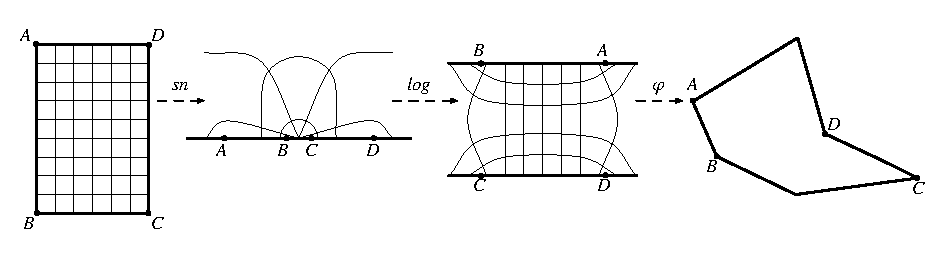
\includegraphics[width=\textwidth]{sc/figs/rectangledia.pdf}
\caption{An example of the series of mappings required to go from the rectangle to an arbitrary polygon using the \sch\ transform. From left to right: the corners of the rectangle are mapped to points on the real line using the Jacobi elliptic function; using a $\log$ transformation, points in the upper-half plane are mapped to the strip (this is purely for computational convenience, this step could be skipped and the \sch\ transform from the upper half-plane to the polygon found); finally, points are mapped from the strip to the polygon via \sch\ transform.}
\label{rectangledia}
\end{figure}

\subsection{Computation of the \sch\ mapping}
\label{sc-mapping-problem}

To compute the map, the prevertices, $w^*_k$ must be found. \label{cor-3s17}As mentioned above, the prevertices are solutions to complicated, non-linear equations and must be found numerically. This section illustrates a simple algorithm for finding the prevertices (the primary reference is \citeb[p. 23--27]{driscoll}).

The complex constants ($A$ and $C$) in the above equations control scaling, translation, and rotation and can \label{cor-r29-3}be computed once the prevertices are found. The $w^*_k$ are found by iteratively by mapping those points back to the polygon to give an approximation to $\Gamma$, $\Gamma^\prime$. To measure the quality of approximation of $\Gamma^\prime$ to $\Gamma$ the following set of equations are used:
\begin{equation}
\label{optimizeme}
F_k = \frac{\vert \varphiinv(w_{k+1}) -  \varphiinv(w_k) \vert}{\vert \varphiinv(w_2)-\varphiinv(w_1)\vert} - \frac{\vert w^*_{k+1} - w^*_k\vert}{\vert w^*_2 - w^*_1\vert} \qquad \text{for } k=3,\dots,K-1.
\end{equation}
Here $\vert \varphiinv(w_{k+1}) -  \varphiinv(w_k) \vert$ is the distance between the $k^{\text{th}}$ and $(k+1)^{\text{th}}$ vertex. This is found by integrating along the line between the points within $W$. See also \secref{algorithmsketch}.

Intuitively, we are comparing the side lengths of the true polygon with its approximation in order to measure how well $\Gamma^\prime$ approximates $\Gamma$ at each iteration (\cite[A-3]{snider}). Both of these measures are scaled by the distance between the first two vertices (in their respective domains).

Note that \eqn{optimizeme} does not include the vertex $w_K$. By theorem 3.1 of \cite[p. 24]{driscoll} a polygon is precisely defined by its angles and its vertices not including $w_K$ (since if the direction of the edges leaving $w_1$ and $w_{K-1}$ are known, the point where they meet may be found). It is for this reason, in the upper half-plane case, that $w_K$ can be mapped to $\infty$ without loss of generality.

Also note that \eqn{optimizeme} does not include $w_1$ or $w_2$ in the numerator on the right hand side. This is due to all vertices (and hence $w_1$ and $w_2$) being rescaled, rotated, and translated by the complex constants, $A$ and $C$, in the \sch\ formula.

\label{cor-3s18-2}In practice some of the prevertices are fixed. For the rectangle case, the vertices of $\Gamma$ which will map to which vertices of the rectangle must be specified (\cite[p. 48]{driscoll}). In the unit disc case $w^*_K, w^*_{K-1}$ and $w^*_{K-2}$ are fixed as $w^*_K=1$, $w^*_{K-1}=-i$ and $w^*_{K-2}=-1$ (\cite[p. 24]{driscoll}). 

The scaling factor, $C$, may be calculated using:
\begin{equation}
C=\frac{\vert \varphiinv(w_2)-\varphiinv(w_1)\vert}{\vert w_2 - w_1\vert}.
\end{equation}
\label{cor-r29-6}\label{cor-3s19}%If $C$ is not calculated then it is known that $\Gamma$ and $\Gamma^\prime$ are similar (in the geometric sense) and so the mapping is correct up to scaling and rotation. 

$A$ is the image of the base point of the integration and is usually written as $w_0$. For computational reasons this is usually the prevertex nearest to the point which is to be mapped\label{cor-3s18-1}, $w^*$ (\cite[p. 27]{driscoll}).


\subsubsection{Sketch of an algorithm to calculate the \sch\ mapping}
\label{algorithmsketch}
\label{cor-e7}
\begin{enumerate}
\item Accept inputs:
   \begin{itemize} 
      \item $w_1,\dots,w_K$ (the vertices of $\Gamma$),
      \item $K$ (the number of vertices),
      \item $\alpha_1,\dots,\alpha_K$ (the internal angles at each vertex, divided by $\pi$),
      \item \label{cor-3s20}$w^*_1,\dots,w^*_K$ (initial values for the prevertices),
      \item $\epsilon$ (tolerance for convergence).
   \end{itemize}
\item Define the objective function, $F_k$, as:
 \begin{equation*}
F_k=\frac{\vert \varphiinv(w_{k+1}) -  \varphiinv(w_k) \vert}{\vert \varphiinv(w_2)-\varphiinv(w_1)\vert} - \frac{\vert w^*_{k+1} - w^*_k\vert}{\vert w^*_2 - w^*_1\vert}, \qquad \text{for } k=3,\dots,K-1,
 \end{equation*}
\begin{enumerate}
\item Use steepest descent and then Newton's method to minimize each of the $F_k$s with respect to $w^*_k$ for each $k$.
\item Update $w^*_1,\dots,w^*_K$.
\item Go back to (a) unless $\vert F_k \vert < \epsilon \quad \forall k$. 
\end{enumerate}
\item Calculate $C$ and $A$ as detailed above.
\item Return values for $w^*_1,\dots,w^*_K$, $C$ and $A$.
\end{enumerate}

Starting values for the algorithm are evenly spaced vertices around the edge of the disc/rectangle or, in the case of the plane, along the real line. Not including those vertices specified as being fixed, above.

\subsection{Moving between $W$ and $W^*$}

\subsubsection{Forwards map}

Calculating the forwards map is simply a case of evaluating $\varphi$ at the necessary points. Definitions of the forwards mappings are given in \secref{schparprob}.

\subsubsection{Backwards map}
\label{sc-backwardsmap}

To calculate the backwards mapping, there are two possible approaches: (i) using Newton's method to solve the equation $\varphi(w^*)-w=0$ and (ii) solving the initial value problem (IVP):
\begin{equation}
\label{scivp}
\frac{dw^*}{dw}=\frac{1}{\varphi^{-1}(w^*)} \quad \text{and} \quad \varphiinv(w_0)=w^*_0.
\end{equation}
In practice a combination of these methods are used. Solving \eqn{scivp} approximately gives the starting values for the Newton iterations which are significantly faster (since $\varphi^{-1}$ is cheaper than $\varphi$ to compute) (\cite[p. 29]{driscoll}).

The only problem with this is that the path from $w_0$ to the point to map, $w$, must lie entirely inside the polygon. Whether this is true is not known, since after the mapping has been computed the only known points are the vertices (at which the IVP is singular). So, to combat this, all points on the path are checked sequentially. This computation, although inelegant, is fast compared to the IVP/Newton iterations.

An example of using the backwards map to find the transformed co-ordinates from a square to the unit disc is given in \fig{squaredomain}. An irregular nonagon is given in \fig{irregdomain}. Note that in these two diagrams the CRDT method described in \secref{sc-crdt} was used rather than the method given in \secref{sc-mapping-problem} where the three vertices are fixed on the circle.


% Square domain mapping diagram
\begin{figure}[t]
\centering
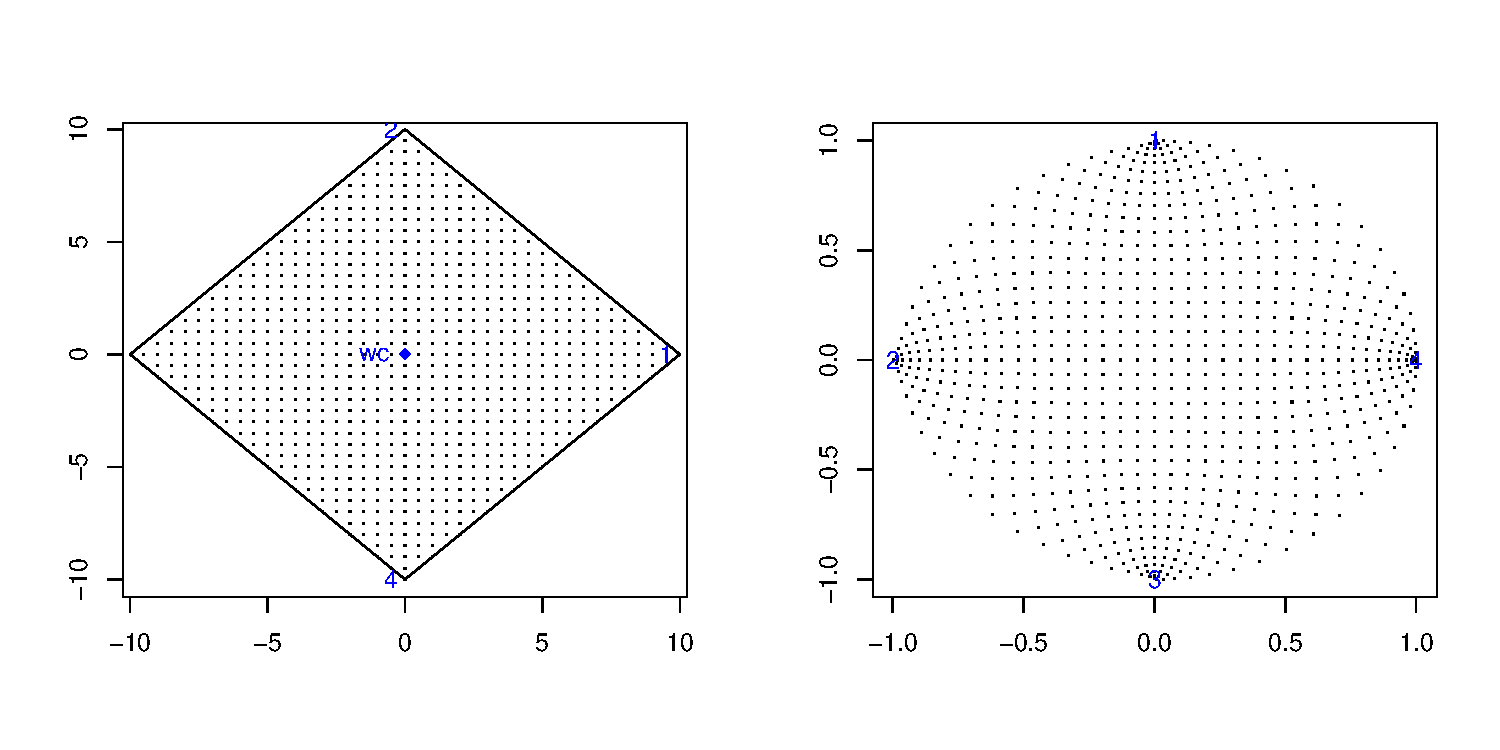
\includegraphics[scale=0.5]{sc/figs/squaredomain.pdf}
\caption{A regular grid of points over the square region (left). The right panel shows the mapping of these points under the \sch\ transformation to the unit disc using the CRDT method described in \secref{sc-crdt}.}
\label{squaredomain}
\end{figure}

% Irregular mapping diagram
\begin{figure}[t]
\centering
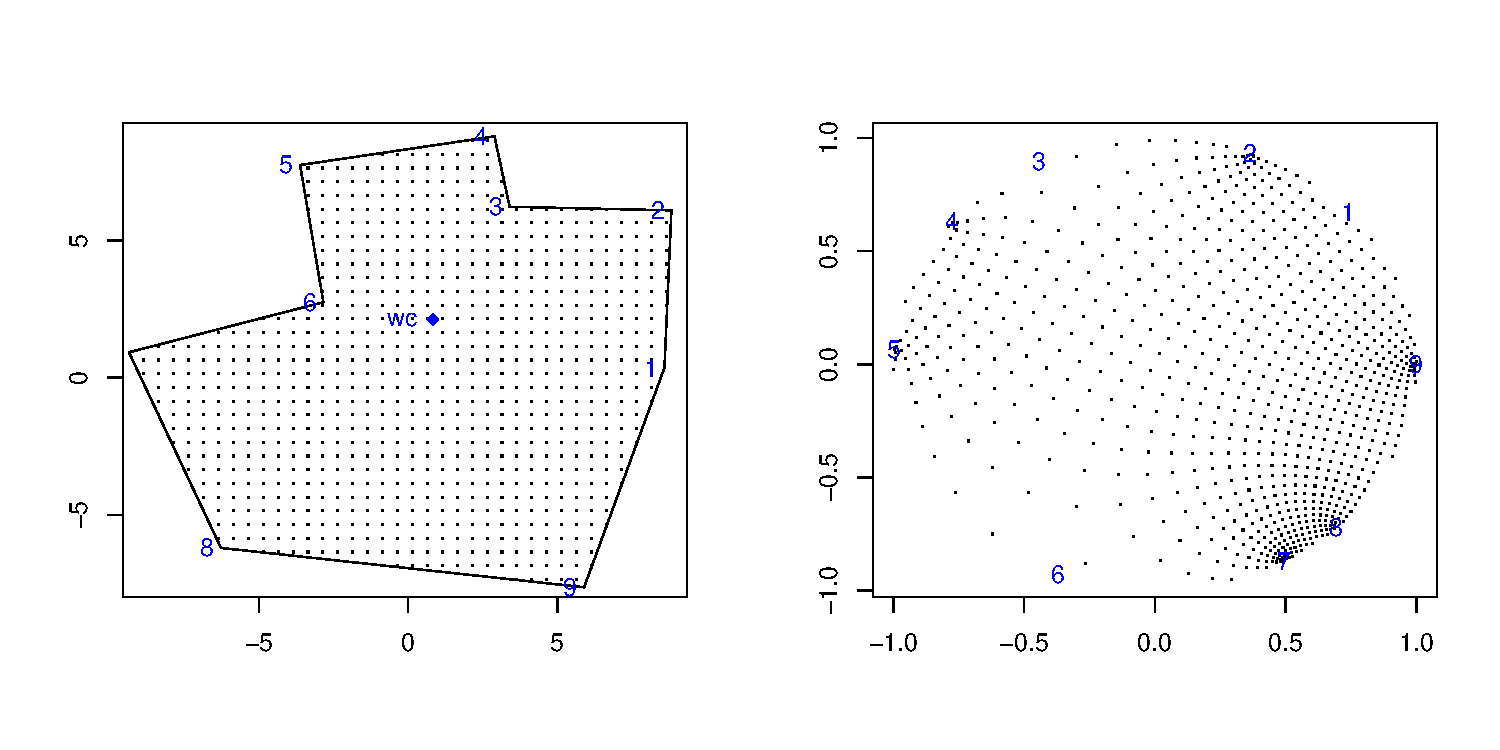
\includegraphics[scale=0.5]{sc/figs/irregulardomain.pdf}
\caption{A regular grid of points over region bound by a irregular nonagon (left). The right panel shows the mapping of these points under the \sch\ tranformation to the unit disc using the CRDT method described in \secref{sc-crdt}}
\label{irregdomain}
\end{figure}

\subsection{Crowding}
\label{sch-crowding}

\subsubsection{The crowding problem}

When the polygon is elongated or has many vertices, the mapped vertices may be positioned too closely in the transformed domain. In elongated regions prevertices can be located exponentially close such that they are indistinguishable in finite precision arithmetic (\cite{howell90}). This effect is referred to as \emph{crowding} and can be observed in \fig{crowdeddisk}. 

% Crowded mapping diagram
\begin{figure} [tbp]
\centering
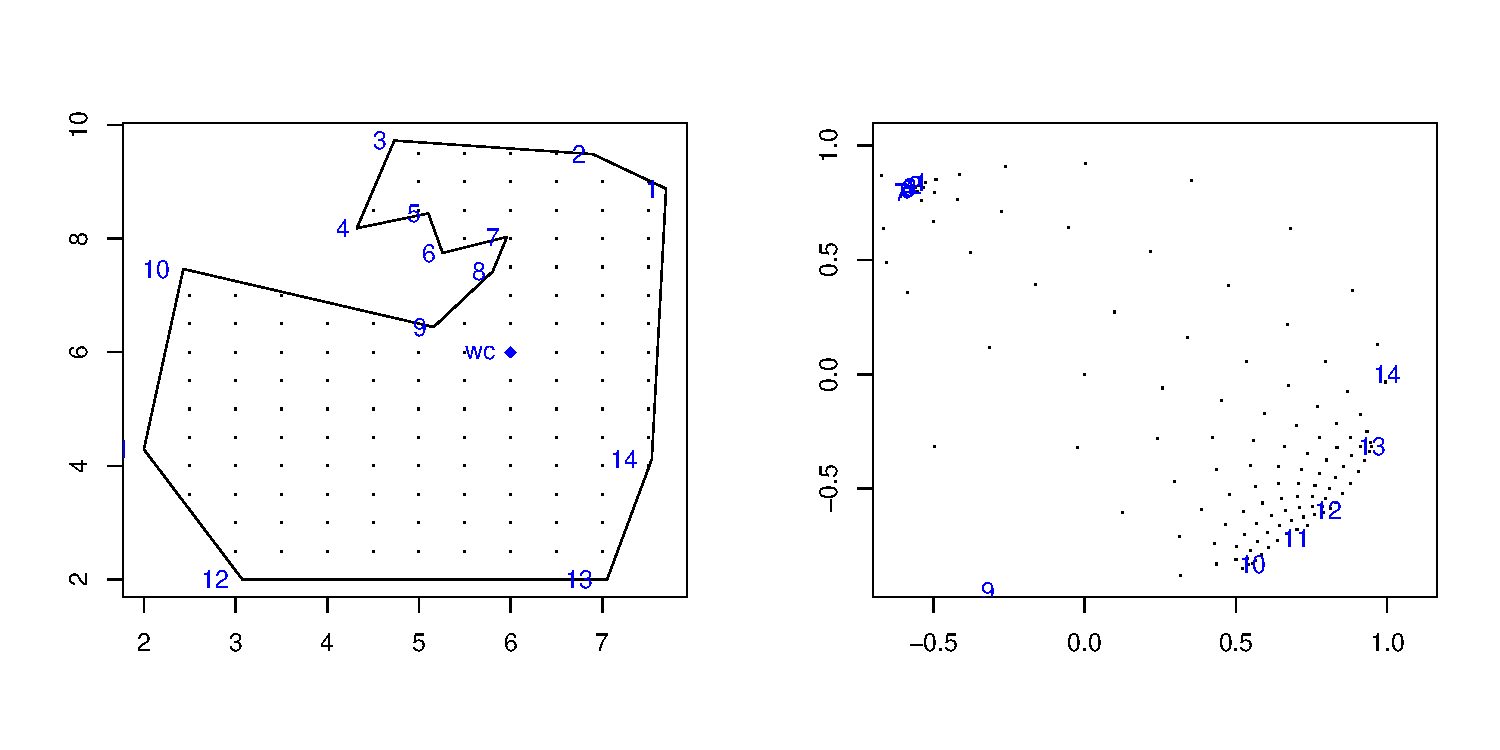
\includegraphics[scale=0.5]{sc/figs/crowdeddisk.pdf}
\caption{An example of crowding. Note that prevertices 1 through 8 are mapped almost to a singularity in the right panel.}
\label{crowdeddisk}
\end{figure}

\subsubsection{Fixing crowding}
\label{sc-crdt}

If the crowding is caused by $\Gamma$ being elongated then a  primitive fix is to map to an elongated domain such as the rectangle or plane. This approach is suggested in \citeb{howell90}, however, as they point out, this does not eliminate all crowding and problems can still occur when there are acute peninsulae in the polygon. Mapping to an elongated domain also does not fix problems which occur when mapping from T- or H-shaped domains (so-called ``multiply elongated'' domains).

In order to combat this problem more effectively, \citeb{vavasis96} propose the CRDT (cross-ratios of the Delaunay triangulation) algorithm (see below). The CRDT algorithm replaces step 2 in the algorithm described in \secref{sc-mapping-problem}. 

In the solution to the \sch\ parameter problem given in \secref{sc-parprob}, conditions on the side lengths and orientations of the polygon are enforced. The CRDT algorithm imposes conditions about quadrilateral sections of the polygon and the diagonals of the polygon. First a Delaunay triangulation of the domain is performed and then pairs of triangles are merged into quadrilaterals. A measure is then defined (the \emph{cross-ratio}) which specifies a set of non-linear equations to be solved. These equations enforce the constraint that the cross-ratio in mapped polygon comes out correctly. 

\citeb{vavasis96} also note that each set of prevertices has $K-3$ degrees of freedom, hence there is a three parameter family of possible vertex arrangements that all map to the same polygon. The most stable of these embeddings should be used. This idea can be extended by noting that the polygon is identical when additional vertices are added between the current ones, provided that the internal angle associated with the new vertex is $\pi$. These extra vertices also do not change the \sch\ formula since in (\ref{unitscmap}) $\alpha_k=1$ for an angle of $\pi$. Adding these extra vertices gives control over the aspect ratio of the mapping.

Putting all of these ideas together gives a replacement for the algorithm described in \secref{sc-mapping-problem}: the CRDT algorithm (\cite[pp. 30-39]{driscoll}). First adding edges to the polygon with internal angle $\pi$ to remove elongated parts of the domain and once the domain is triangulated the cross-ratio is found:
\begin{equation}
\rho(a,b,c,d) = \frac{(d-a)(b-c)}{(c-d)(a-b)},
\end{equation}
for each of the $K-3$ quadrilaterals in the polygon (where $a,b,c,d$ are prevertices). Then, analogously to \eqn{optimizeme} a series of equations are set up specifying that the cross-ratios remain the same in the polygon and the transform of the rectangle back to the polygon. Then solving for the values of $\rho$ for the original domain in the same manner as we solved for side lengths in the original problem. 

In \fig{uncrowdeddisk} the CRDT method is used with a rectangular domain, crowding has been alleviated to some degree. The point density, as well as vertex density seems to be more uniform than in \fig{crowdeddisk}.

% Uncrowded mapping diagram
\begin{figure} [tbp]
\centering
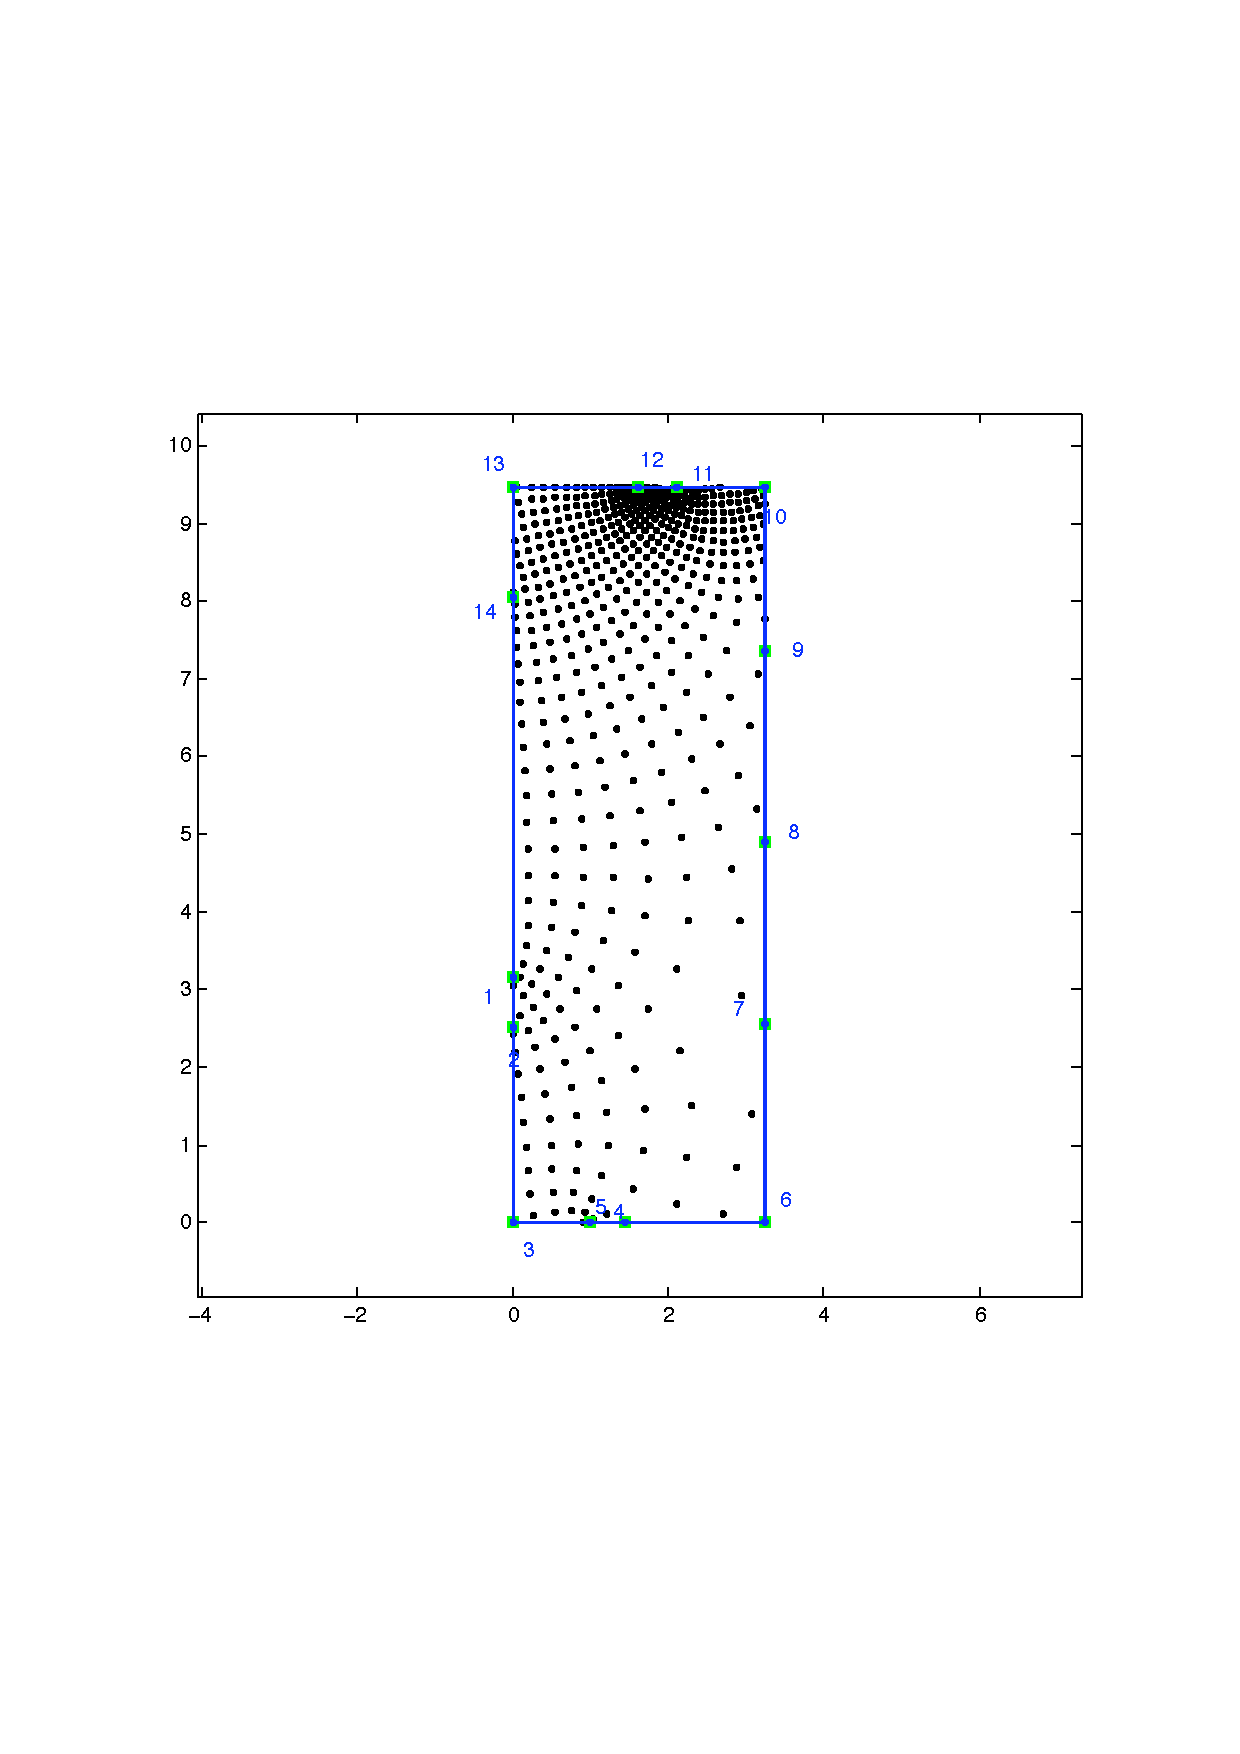
\includegraphics[scale=0.5]{sc/figs/irregular-fixed-crdt.pdf}
\caption{The mapping of the irregular domain featured in \fig{crowdeddisk} using the CRDT method mapping to a rectangle. The crowding is now much less severe.}
\label{uncrowdeddisk}
\end{figure}

The downside of using CRDT is that it may add too many vertices to maintain the aspect ratio, so the algorithm takes longer to run than the one specified in \secref{algorithmsketch} since it tends to be cubic in the number of vertices (\cite{driscoll05}). 

\section{Simulation experiments}
\label{sc-sims}

In order to test the efficacy of the \sch\ transform for the purposes of smoothing over complex regions, a series of simulation experiments were performed. The \emph{SC Toolbox} for MATLAB was used to transform and map the points. Smoothing was then performed in \textsf{R} using the packages \texttt{mgcv} and \texttt{soap}.

\subsection{Ramsay horseshoe}

The first set of simulations were run using the Ramsay horseshoe (see \secref{ramsayfunc}). In order to map as simple a domain as possible, initially a bounding box was used as the $W$ domain and mapped  to the rectangle via the \texttt{evalinv()} function in the \emph{SC Toolbox}. The bounding box is shown in figure \ref{hswithboundingbox}.

\begin{figure}
\centering
% trim order l b r t
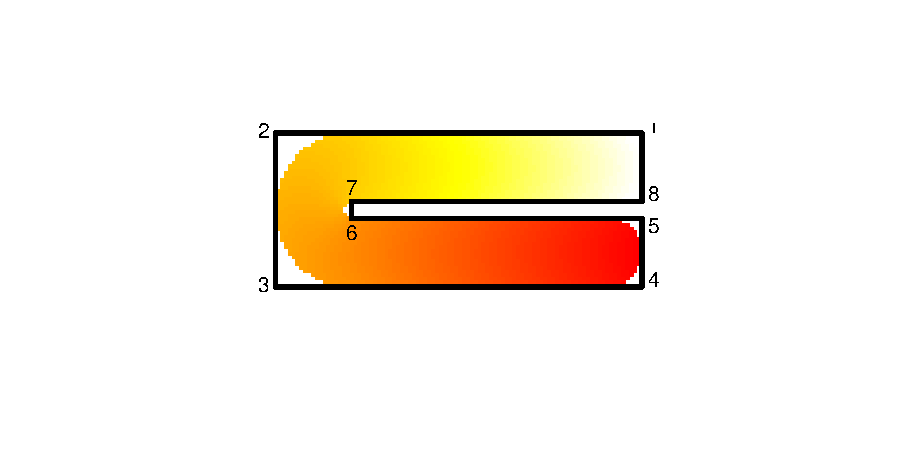
\includegraphics[trim=0.5in 1in 0in 0.5in]{sc/figs/hswithboundingbox.pdf} \\
\caption{The horseshoe with its bounding box. The vertices marked 1, 4, 5 and 8 were mapped to the corners of the rectangle.}
\label{hswithboundingbox}
% generated by /phd-smoothing/sc-writeup/figs/hswithboundingbox.R
\end{figure}

A sample of 1000 points was then taken from the horseshoe and noise added to the data. First the coordinates of the sampled points were expressed as complex numbers of the form (i.e. $w=x_1+ix_2$). The sample was then mapped into $W^*$, creating a new set of coordinates ($w^*=x_1^*+ix_2^*$). Smoothing was then performed over the responses in the $W^*$ domain using the \texttt{gam()} function in \texttt{mgcv} having taken the real and imaginary parts of each data points to be its coordinates. 

The models that were fitted to the samples were as follows:
\begin{enumerate}
\item \textit{soap}: the soap film smoother with 32 internal knots and 30 boundary knots.
\item \textit{sc+ps}: \sch\ transform of the horseshoe's bounding polygon to the rectangle, P-splines with a $6 \times 10$ grid of knots.
\item \textit{sc+tp}: \sch\ transform of the horseshoe's bounding polygon to the rectangle, thin plate regression splines with a maximum basis size of 30.
\item \textit{tprs}: thin plate regression splines with a maximum basis size of 30.
\end{enumerate}

\begin{figure}[t]
\centering
% trim order l b r t
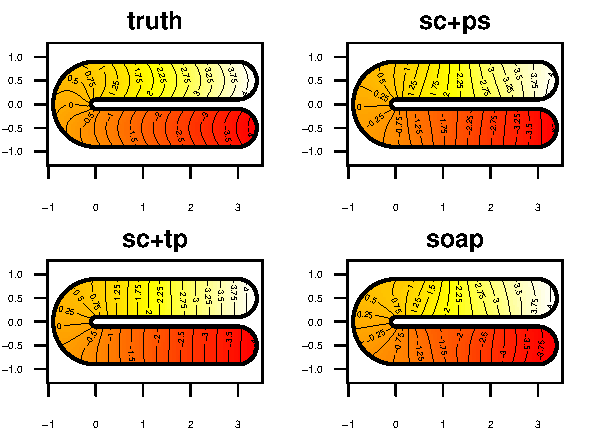
\includegraphics[width=\textwidth]{sc/figs/compsmooth.pdf} \\
\caption{A typical set of predictions using P-splines on the transformed domain (top right, ``sc+ps''), \tprss\ on the transformed domain (bottom left, ``sc+ps'') and soap film smoother (bottom right, ``soap'') for the Ramsay horseshoe (top left, ``truth''). Sample size was 250, the standard deviation of the Gaussian noise added to the samples was set to 1.}
\label{compsmooth}
% generated by figs/pspline.soap.comp.hs.R
\end{figure}

\Fig{compsmooth} shows the true function and typical realisations of: the fit given by a \tprs\ on the transformed domain, a P-spline fit on the transformed domain and the fit given by the soap film smoother. Looking at the heat maps one can see that the general shape of the horseshoe function is clearly being reproduced by all methods (especially in comparison to that in \fig{leakage}). However, on the transformed domains the curvature across the minor axis is not captured.

\begin{table}[tb]
\centering
\begin{tabular}{c c}\\
Sample size & Noise level \\
\hline
1000 & 0.3 \\
500 & 0.3 \\
250 & 0.3 \\
100 & 0.3 \\
1000 & 0.5 \\
1000 & 1 \\
1000 & 2 \\
\end{tabular}
\caption{Setup for the simulations using the \sch\ transform for the Ramsay horseshoe. Noise level is the number a random deviate from a standard Normal distribution was multiplied by before being added to the value from true test function.}
\label{scramsimtable}
\end{table}

\Tabref{scramsimtable} shows the settings for noise level and sample size of the simulations. Figure \ref{sc-ram-boxplot} shows boxplots of the logarithm of the MSE for the simulations. The \sch\ transform yields results which are comparable, if not better, than the soap film. At a sample size of 100 performance degrades for all methods. 

The fits on the transformed domain and the soap film have much smaller MSE than the \tprs, except in one case, \sch\ with P-splines for sample size 100 and noise level 0.3. Looking closer at the results for this model, there were two results where the MSE was 54.68 and 437.99 which, when removed, put the MSE back to 0.03003, which seems much more reasonable. These results were presumably due to the P-splines' gridded knot setup, giving a poor fit where there was not enough data. This shows one of the many disadvantages of a knot-based approach. These results were removed for the plotting of the boxplots.

\begin{sidewaysfigure}
\centering
% trim order l b r t
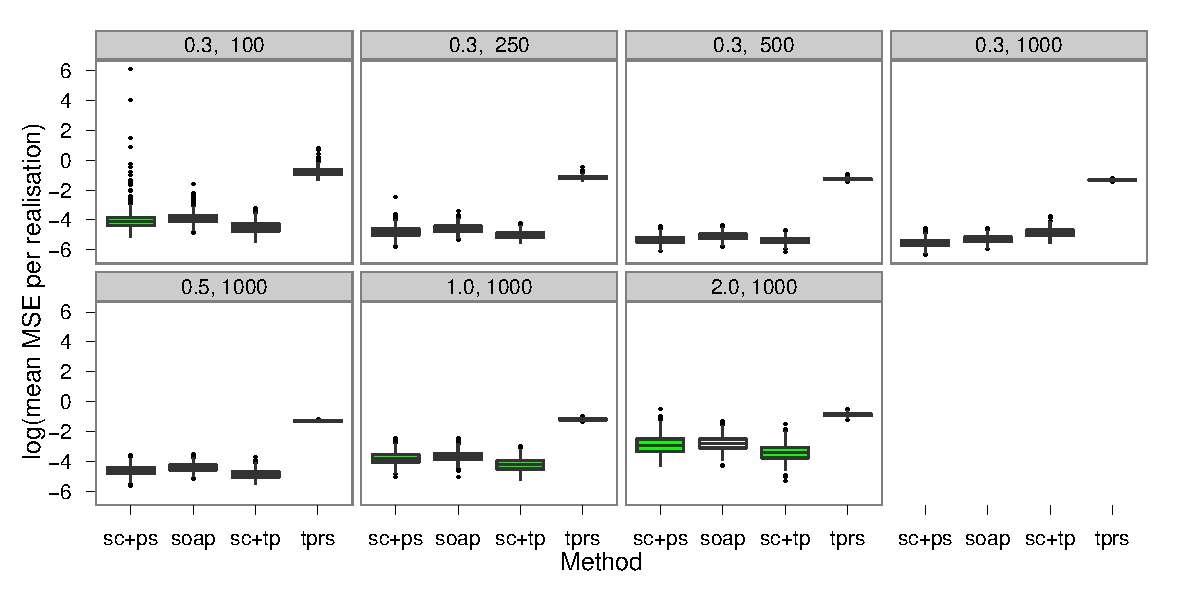
\includegraphics{sc/tablecode/ramsay-boxplot.pdf} \\
\caption{Boxplots of the logarithm of the per-realisation MSE for the simulations on the Ramsay horseshoe for the \sch\ transform method using P-spline (``sc+ps'') and \tprss\ (``sc+tp''), the soap film smoother (``soap'') and \tprss\ (``tprs'') at varying (noise level, sample size) pairings. Colour codings give the results of a Wilcoxon signed rank test on the paired MSEs, between the soap film and the other methods; red indicates significantly worse results, green significantly better and white no significant (at the 0.01 level) difference. In all cases \tprss\ were significantly worse than the soap film smoother.}
\label{sc-ram-boxplot}
% generated by sc/tablecode/ramsay-boxplots.R
\end{sidewaysfigure}


Although this seems initially encouraging, it is worth bearing in mind at this point that in domains like the horseshoe it is obvious what the transform should be. This can be seen by looking at the predicted values for the model in the $W^*$ domain. \Fig{hsvisgam} shows predictions from the fitted surface alongside the true values when the domain has been put into its ``natural'' coordinate system. The coordinate system for the fitted values is the \sch\ transformed coordinates and for the true values it is the major and minor axes of the shape (i.e. one axis along the central curve of the shape and the other perpendicular to that). In the plot, the strong linear trend along the major axis of the horseshoe can be seen in both cases, making this a rather simple smoothing problem for the method. The smooth is being calculated in a close approximation to its natural domain. Such an approximation would not be as easy to find for a less regular, more realistic domain.

\begin{figure}[t]
\centering
% trim order l b r t
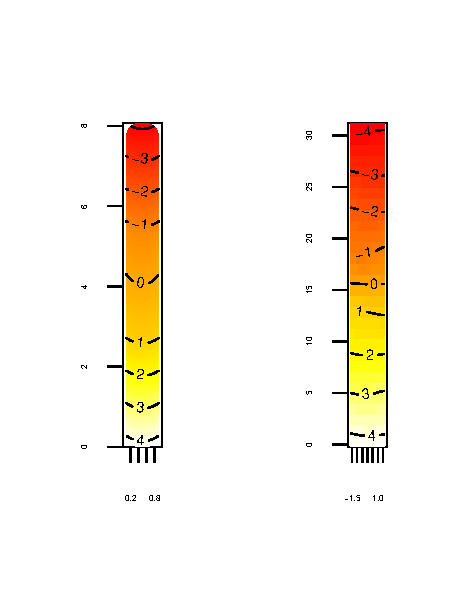
\includegraphics{sc/figs/hsvisgam.pdf} \\
\caption{Heat map of the true values of the modified Ramsay horseshoe projected into its natural domain (left) and the predicted values of the fit given using the \sch\ transform and then smoothed using a \tprs\ (right).}
\label{hsvisgam}
% generated by /phd-smoothing/thesis/sc/figs/hsvisgam.R
\end{figure}

\subsubsection{Alternate Ramsay horseshoe}
\label{sc-alt-horsehoe}

The second domain tested was the alternate version of the Ramsay horseshoe from \citeb{soap}. For this domain there is a gorge running along the major axis of the horseshoe (see \fig{altramsayhorseshoe}). The same simulation setup was used as for the first domain (see table \ref{scramsimtable} and model list, bove).

\begin{figure}[t]
\centering
% trim order l b r t
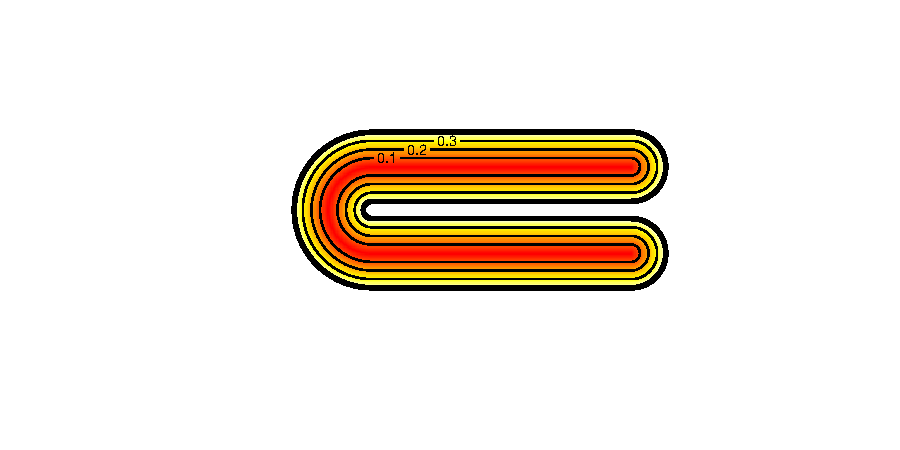
\includegraphics[trim=0.5in 1in 0in 0.5in]{sc/figs/altramsayhorseshoe.pdf} \\
\caption{The alternate version of the Ramsay horseshoe. Unlike the previous horseshoe there is a gorge running along the major axis of the shape.}
\label{altramsayhorseshoe}
\end{figure}

Simulation results for the alternative horseshoe begins to see the soap film creep ahead of the transformation method. The boxplots in figure \ref{sc-altram-boxplot} show that the combination of \sch\ transform and P-splines performs better than the soap film when the sample size is low, however at higher noise levels and sample sizes the soap film smoother begins to out-perform the transform method.

Figure \ref{altramsaycomp} shows that the \sch\ mapping with P-splines captures the overall structure of the shape better than the soap film smoother, which is rather patchy in its reproduction of the alternate horseshoe. Although the P-spline fit ignores the gradient at the ends of the shape. The \sch\ with \tprs\ basis appears worst here, not capturing any of the main features of the domain.

\begin{sidewaysfigure}
\centering
% trim order l b r t
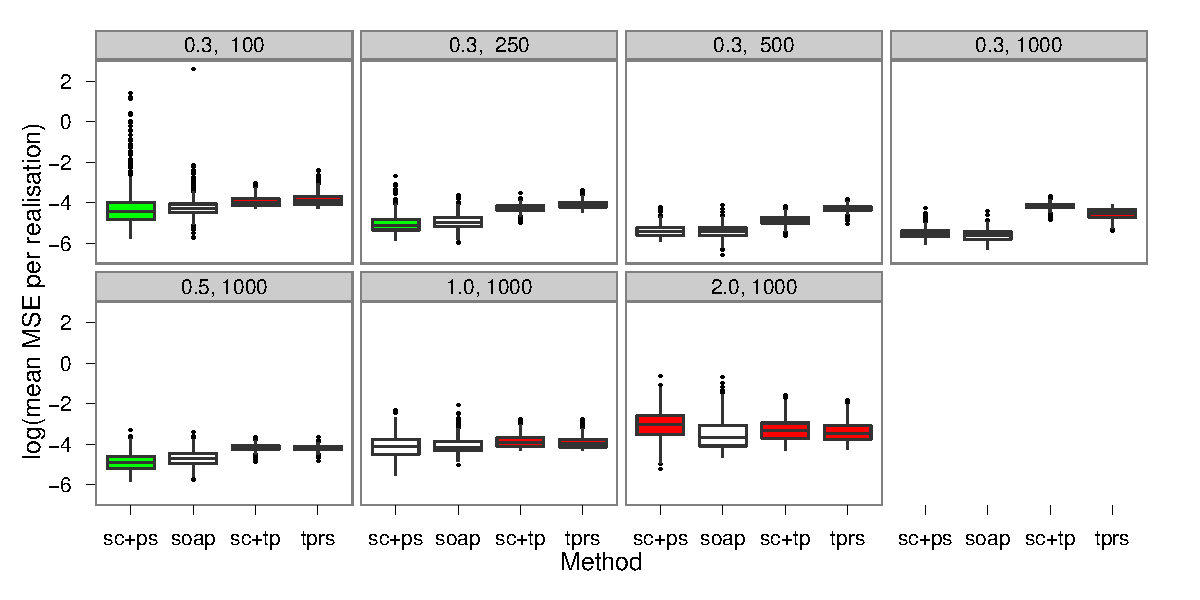
\includegraphics{sc/tablecode/altramsay-boxplot.pdf} \\
\caption{Boxplots of the logarithm of the per-realisation MSE for the simulations on the alternate Ramsay horseshoe for the \sch\ transform method using P-spline (``sc+ps'') and \tprss\ (``sc+tp''), the soap film smoother (``soap'') and \tprss\ (``tprs'') at varying (noise level, sample size) pairings. Colour codings give the results of a paired Wilcoxon signed rank test to detect the difference in MSE between the soap film and the other methods; red indicates significantly worse results, green significantly better and white no significant difference (at the 0.01 level).}
\label{sc-altram-boxplot}
% generated by sc/tablecode/ramsay-boxplots.R
\end{sidewaysfigure}


\begin{figure}[t]
\centering
% trim order l b r t
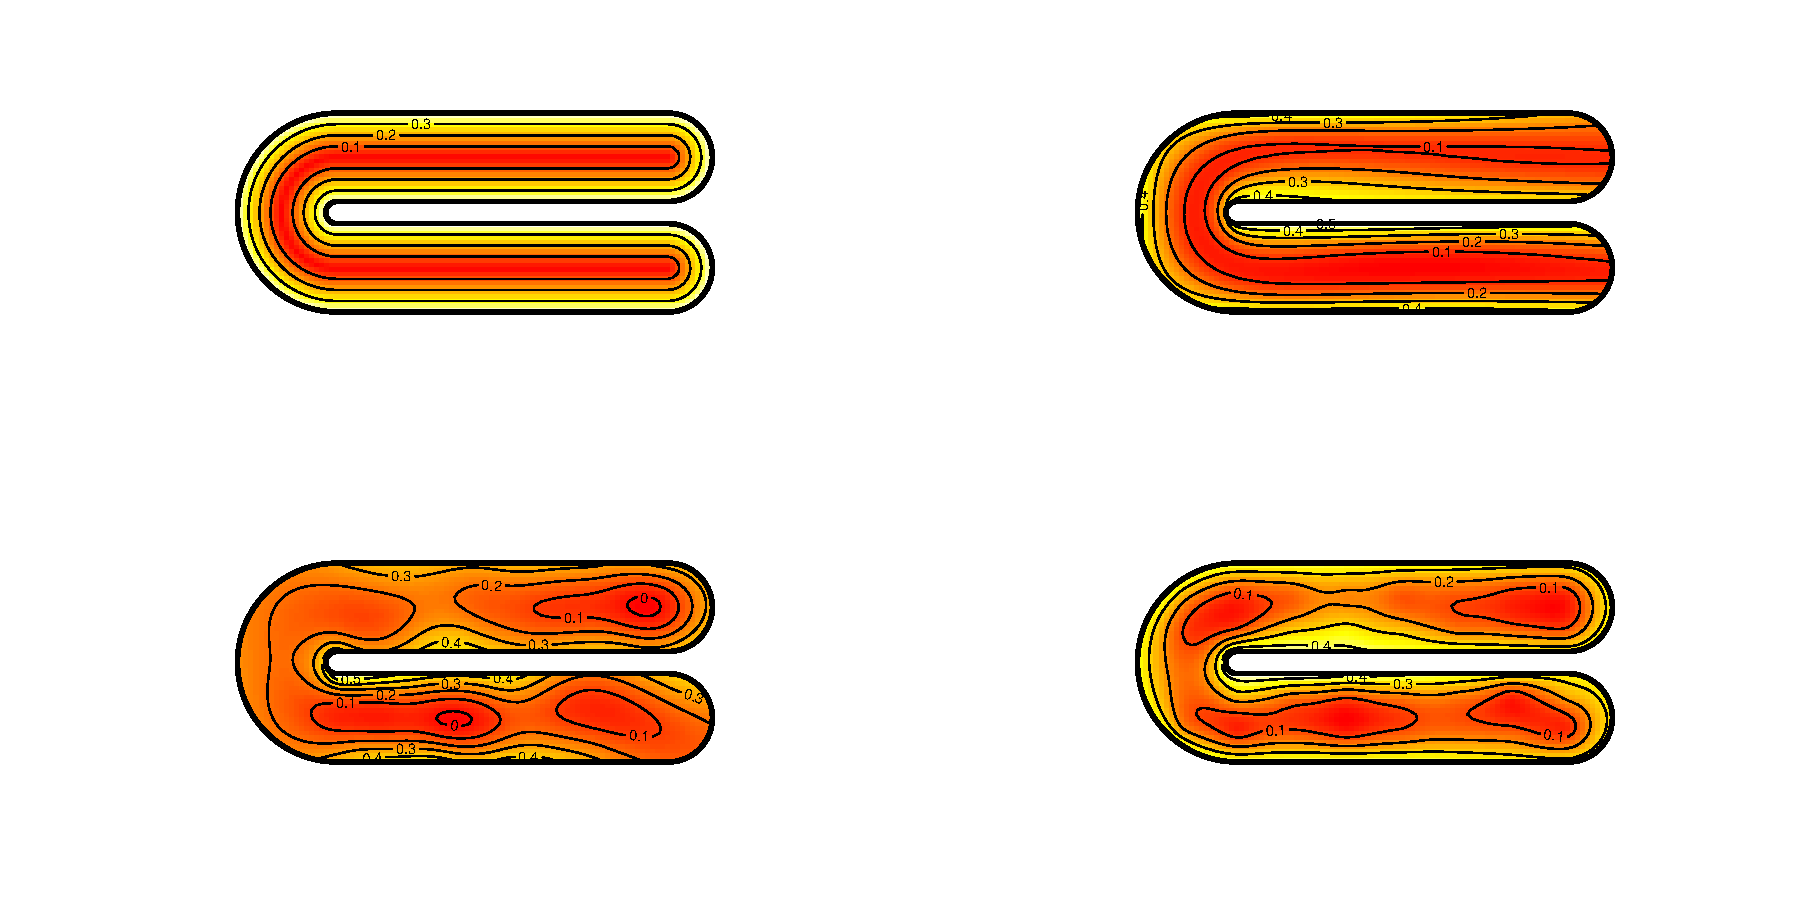
\includegraphics[width=6in]{sc/figs/altramsaycomp.pdf}\\
\caption{Typical realisations of the fit to the alternate Ramsay horseshoe for each method. Clockwise from top left: the original figure (``truth''), the function estimated by the \sch\ transform with P-splines (``sc+ps''), function estimated by the \sch\ transform with \tprss\ (``sc+tp'') and finally the soap film smoother (``soap''). Additive noise level was 1.}
\label{altramsaycomp}
% generated by /phd-smoothing/sc-writeup/figs/altramsaycompare.R 
\end{figure}


\subsubsection{The effect of the \sch\ transform on the domain}

Using the \sch\ transform before smoothing gives an increase in performance for some smoothers in some situations but not others. To investigate the effect of the distortion on the domain, the mapping of a straight line in the $W$ domain can be plotted along with its equivalent line in the $W^*$ domain. It is also useful to look at the response along that line in both the transformed and untransformed coordinate systems and see how this compares to looking at the response in the horseshoe's natural coordinate system.

\begin{figure}[t]
\centering
% trim order l b r t
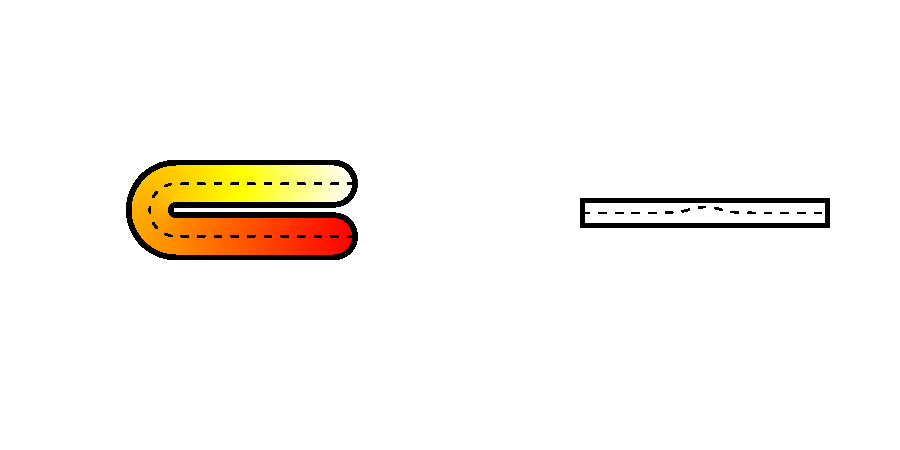
\includegraphics[trim=0.5in 1in 0in 1in]{sc/figs/horseshoecentreline.pdf} \\
\caption{Mapping of a straight line along the major axis of the Ramsay horseshoe to its position in the ``unwrapped'' domain.}
\label{horseshoecentreline}
% generated by /phd-smoothing/thesis/sc/nullspace.test.R 
\end{figure}

\Fig{horseshoecentreline} shows a line along the centre of the horseshoe and its equivalent line in the transformed domain. We can see from this that a line that is straight in the domain (in the sense that it runs along the major axis, keeping the same distance from either side of the horseshoe) has a bump in it in the transform. The curvature does not appear to be particularly extreme in this case, however, one can imagine that this could get significantly worse for regions with more complicated boundaries.

\Fig{centrelinelineplot} shows the evaluations of the horseshoe function along the line plotted against three coordinates. The first plot shows the function evaluations on the $W$ domain as a response to change in $x_2$. The second on the $W^*$ domain, as a response to $x_2^*$, in the transformed coordinate system. The final plot is in the horseshoe's natural domain, i.e. the value of $f$ as a function of distance along the major axis of the shape. From these plots one can see the quality of approximation to the natural domain of the horseshoe the \sch\ transform provides. Only two minor kinks occur in the line. Looking at where the kinks occur, they correspond exactly to those kinks in \fig{horseshoecentreline}. 

\begin{figure}[t]
\centering
% trim order l b r t
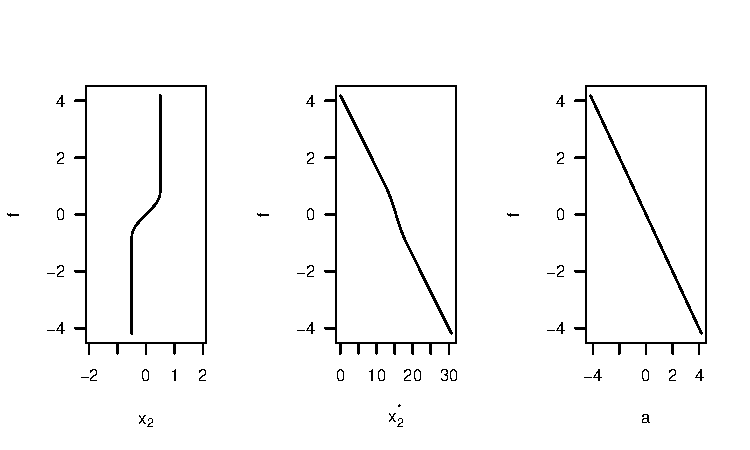
\includegraphics[width=\textwidth]{sc/figs/centrelinelineplots.pdf} \\
\caption{Plots of the horseshoe function against the $y$ axis for (left) the untransformed horseshoe, (middle) the shape under the \sch\ transform and, (right) the function evaluation against the major axis.}
\label{centrelinelineplot}
% generated by /phd-smoothing/ramseysim/nullspace.test.R 
\end{figure}

\Fig{altcentrelinelineplot} shows analogous plots to \fig{centrelinelineplot} for the alternate Ramsay horseshoe and backs up this hypothesis. The second panel shows the mapping of the $x_2$ component of the centreline against the response and the third panel shows the same in the horseshoe's own domain. The two plots appear to be indistinguishable, aside from the change in scale on the horizontal axis; this may account for the failure of the P-splines to model the gradient at the ``ends'' of the shape see in figure \ref{altramsaycomp}.

\begin{figure}[t]
\centering
% trim order l b r t
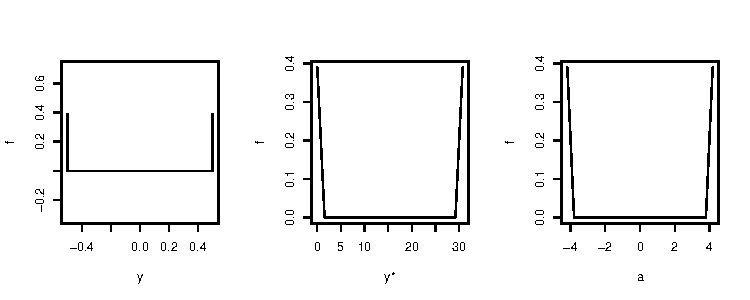
\includegraphics[width=\textwidth]{sc/figs/altcentrelinelineplots.pdf} \\
\caption{Plots of the alternate horseshoe function against the $y$ axis for (left) the untransformed horseshoe, (middle) the shape under the \sch\ transform and, (right) the function evaluation against the major axis.}
\label{altcentrelinelineplot}
% generated by /phd-smoothing/altramsaysim/nullspace.test.R 
\end{figure}

\subsection{Peninsula domain}
\label{sc-penin}

Looking at a more realistic domain highlights potential problems with using the \sch\ transform in practice. The domain in the top left corner of \fig{sc-wigglytop2-real} shows a domain which replicates some of the features of a coastline.

% realization
\begin{figure}[t]
\centering
% trim order l b r t
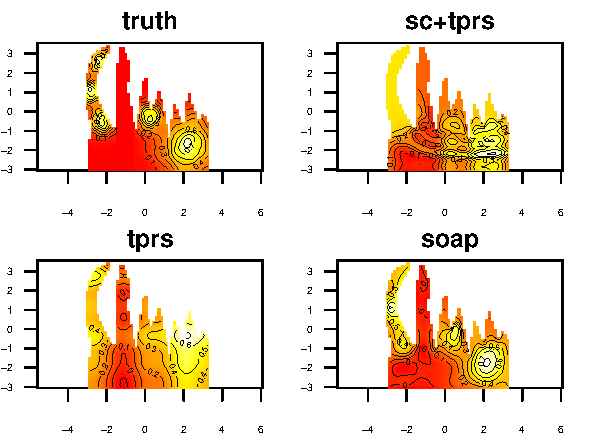
\includegraphics[width=\textwidth]{sc/figs/wigglytop2-real.pdf} \\
\caption{The peninsulae domain. From top left, clockwise: truth, fit from \sch\ transform with \tprs, soap film smoother fit, and \tprs\ fit for typical realisations. Sample size was 500 and the noise level was 0.02. For the \sch\ transformed domains, the rectangular mapping was used.}
\label{sc-wigglytop2-real}
% generated by wigglytop2 fit.irregular.R
\end{figure}

The CRDT algorithm was used for the \sch\ mapping, extra vertices introduced into the polygon with angle $\pi$, are shown, along with the mapping in \fig{wigglytop2-numbered}. From this figure one can see that although there is no crowding in the numerical sense discussed in \secref{sch-crowding}, there is significant ``bunching-up'' of the vertices. This would indicate that odd artefacts might be introduced into the smooth.

Several combinations of vertex mappings and knots were tried. The result of this was that the vertices chosen to map to the corners of the rectangle were those shown in pink in \fig{wigglytop2-numbered}. For the soap film smoother a 15 by 15 grid of internal knots was used, of which 109 were inside the region. The cyclic spline around the boundary used 49 knots. Clearly this is the kind of domain in which the soap film smoother performs well (when the chance of leakage is high).

% wt2 vertex mapping
\begin{figure}[t]
\centering
% trim order l b r t
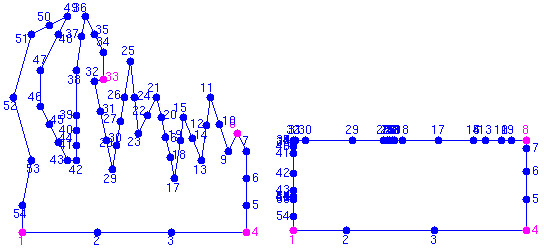
\includegraphics[width=\textwidth]{sc/figs/wigglytop2-numbered.png} \\
\caption{Mapping of the polygon to rectangle for the double peninsula domain example. Note the extra vertices added by the CRDT algorithm.}
\label{wigglytop2-numbered}
% generated by Matlab
\end{figure}

% wt2 point mapping
\begin{figure}[t]
\centering
% trim order l b r t
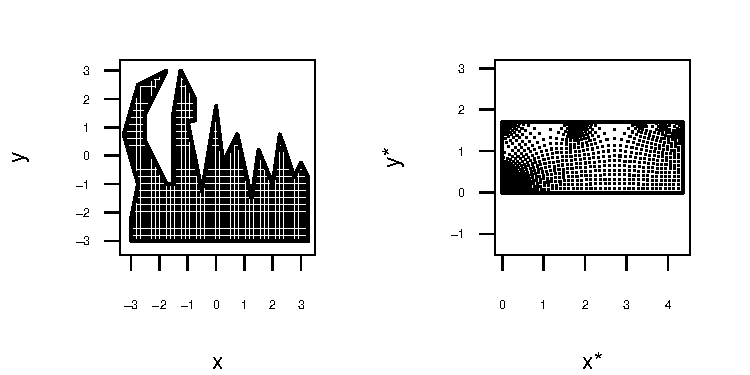
\includegraphics[width=6in]{sc/figs/wt2-points.pdf} \\
\caption{Change in the density of points between the mapped and unmapped spaces for the double peninsula domain. Areas with particularly high density in the right panel correspond to vertices in the left.}
\label{wt2-points}
% generated by thesis/sc/figs/wt2-pointmap.R
\end{figure}

The models used in the simulation were:
\begin{enumerate}
\item \textit{soap}: the soap film smoother with 109 internal knots and 49 boundary knots.
\item \textit{sc+tprs}: \sch\ transform of the peninsula domain to the rectangle, thin plate regression splines with a maximum basis size of 49.
\item \textit{sc+tprs box}: \sch\ transform of the peninsula domain's bounding polygon to the rectangle, thin plate regression splines with a maximum basis size of 49.
\item \textit{tprs}: thin plate regression splines with a maximum basis size of 49.
\end{enumerate}

Looking at the realisations in \fig{sc-wigglytop2-real}, one can see that the \sch\ transform causes a huge distortion in the surface. The contour lines in the upper right pane of the figure show how the distortions have pushed the data points around, causing a very bad fit. It also looks as though there is a ridge across the smooth over the domain, which is clearly unwanted. The \tprs\ and the transform method both smooth over the details in the first peninsula. The soap film smoother is vastly superior to either method in this situation as can be seen in the boxplots in \fig{wigglytop2-boxplots}.

% boxplot
\begin{figure}[t]
\centering
% trim order l b r t
%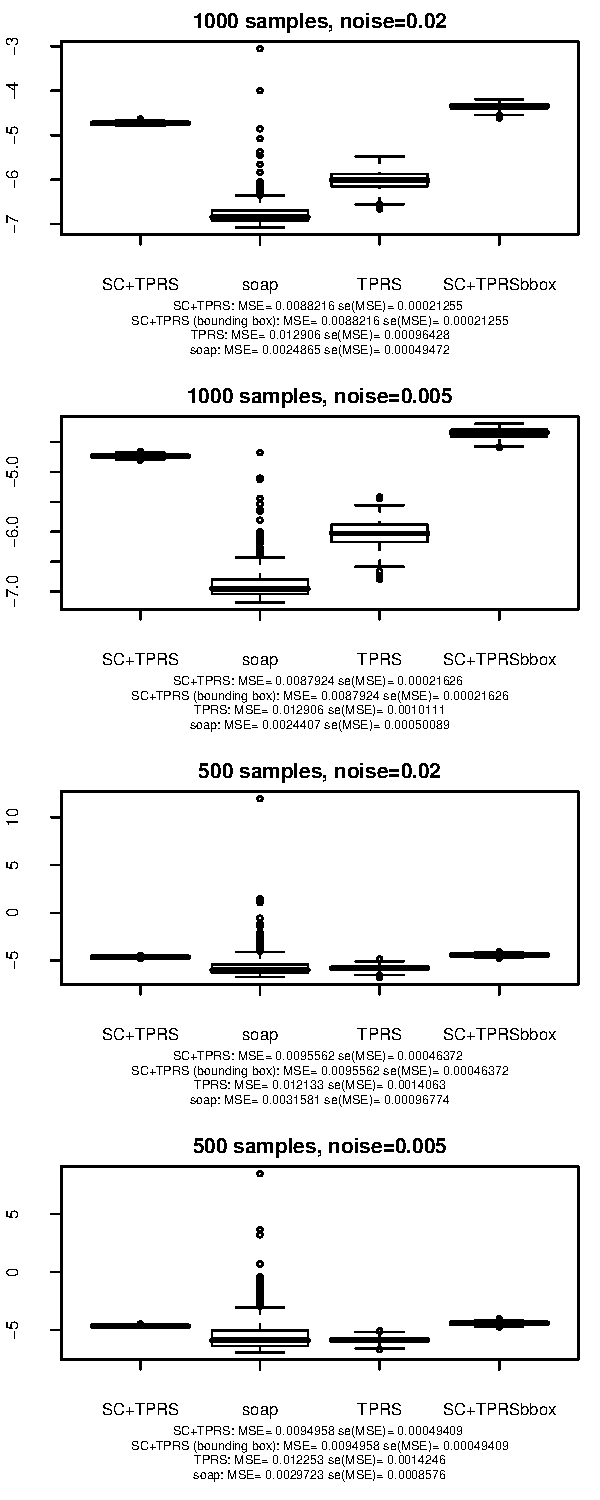
\includegraphics[width=6in]{sc/figs/wigglytop2-boxplot.pdf} \\
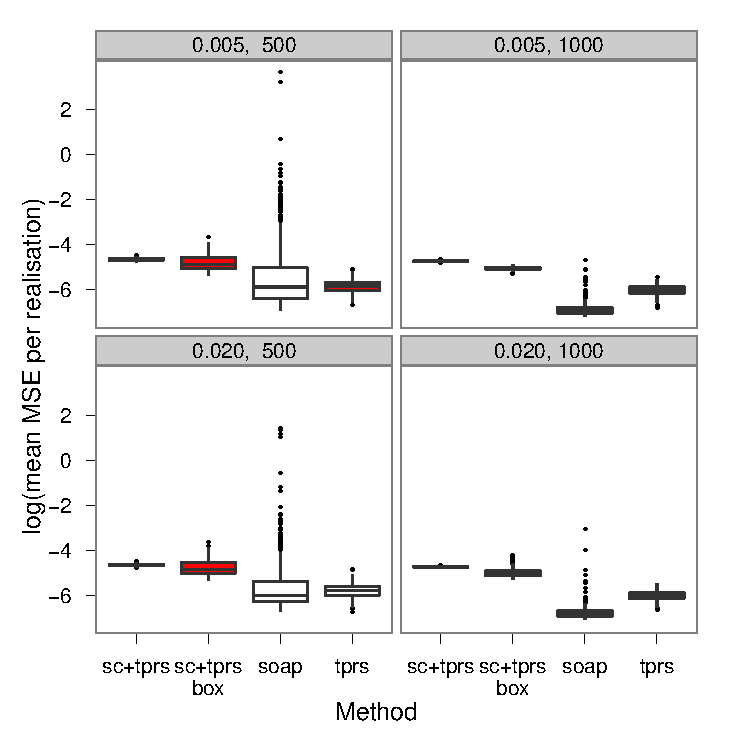
\includegraphics[width=\textwidth]{sc/tablecode/wt2-boxplot.pdf} \\
\caption{Boxplots of the logarithm of the MSE averaged over 1253 prediction points for 500 replicates for various (noise level, sample size) pairs. The models fitted were: the rectangle \sch\ mapping with \tprss\ (``sc+tprs'') and the bounding box mapped to the rectangle (``sc+tprs box''), alongside the soap film smoother (``soap'') and \tprs\ (``tprs''). Colours indicate the results of a paired Wilcoxon signed rank test on whether the MSEs were significantly different from the soap film smoother's; red indicates significant different and worse MSE, white non-significant (at the 0.01 level).}
\label{wigglytop2-boxplots}
% generated by makeboxplots.R
\end{figure}

In the horseshoe simulations the shape of the domain was simplified by using a bounding polygon. \Fig{wigglytop2-boxplots} shows the results of using the bounding polygon shown in \fig{wigglytop2-bbox-numbered} with the \sch\ mapping (again mapping to the rectangle) as  an attempt to reduce the distortions seen in \fig{sc-wigglytop2-real}. There is no significant increase in performance by attempting to use the bounding polygon and in fact the variability in the MSE appears to have increased. Although this did iron out some of the artefacts in the smooth, \fig{wigglytop2-bbox-real} shows that new, undesirable, features appear. It appears that the \sch\ transform does not perform well in such a situation.

\begin{figure}[t]
\centering
% trim order l b r t
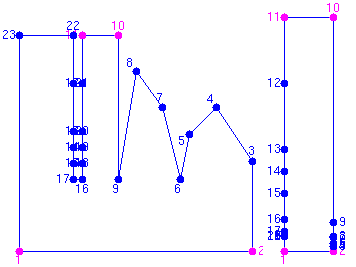
\includegraphics[width=3in]{sc/figs/wigglytop2-bbox-numbered.png} \\
\caption{The CRDT mapping of the bounding box to the rectangle for the peninsula domain. Pink vertices correspond to those mapped to the corners of the rectangle.}
\label{wigglytop2-bbox-numbered}
% generated by Matlab
\end{figure}


% realisation
\begin{figure}
\centering
% trim order l b r t
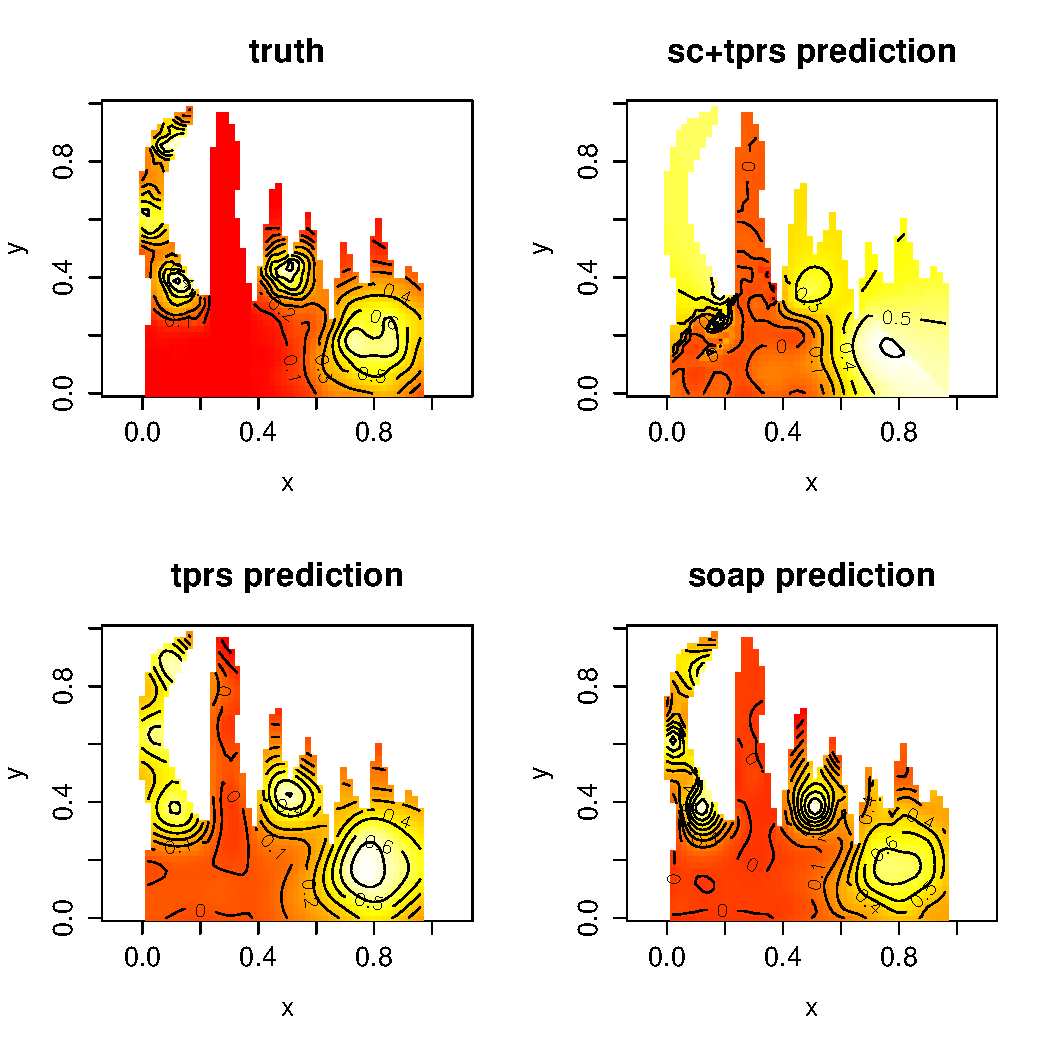
\includegraphics[width=6in]{sc/figs/wigglytop2-bbox-real.pdf} \\
\caption{The domain with two peninsulae. Truth and typical realisations for (clockwise from top right) a \tprs\ fit to the \sch\ transformed domain using the bounding box, the soap film smoother, and a \tprs\ on the untransformed domain. Sample size was 500 and the noise level was 0.02.}
\label{wigglytop2-bbox-real}
% generated by wigglytop2-bbox fit.irregular.R
\end{figure}


\section{Conclusions}
\label{sc-conclusions}

Domain morphing-type techniques undeniably show some promise when it comes to the problem of smoothing over complex regions. Yet the \sch\ mapping is not the correct transformation to use for  all domains. What has been seen here is that the mapping is too prescriptive in its morphing of the domain. There is no reason to think that a particular domain should always be transformed to, it should just be a convenient shape to smooth over. The restriction to only use the unit disc, rectangle, etc. constrains the technique, causing phenomena which are as bad (if not worse) than the leakage we initially sought to avoid.

Crowding (in a technical sense) can be avoided by using the CRDT algorithm, but the squashing together of the points caused by using the \sch\ transform causes huge problems when smoothing. This fundamental problem of mapping between domains is exacerbated by using a restricted set of shapes to map into. It would be preferable to minimize the distortion to the distribution of points in space and using a less regular domain for $W^*$, rather than having a pre-specified domain, which causes the distribution o of the points to become concentrated at a few points.

The point map in figure \ref{wt2-points} shows that the \sch\ transform can clearly separate parts of the domain, drawing apart those areas of the domain which were causing the leakage previously. In the case of the Ramsay horseshoe, the transformation that is needed is obvious; problems occur when the transformation is not obvious. With the peninsula domain, it is not clear what an appropriate domain to map into would look like even if the \sch\ transform could map to an arbitrary shape. Certainly, the rectangle or unit disc are not the shapes which immediately come to mind.

Fortunately, all is not lost. This brief foray into conformal mapping has provided plenty of insights into how smoothers will act under mapping schemes. It has also given an appreciation of the criteria which dictate the utility of a transformation-based method, especially with regard to how smoothing behaves when space is distorted.

With these points in mind, the next step is to find a general mapping scheme for domains with complicated boundaries which is not too prescriptive, causes minimum distortions to the distribution of space but minimises the effects of leakage. This is the subject of the following three chapters.



